\documentclass[a4paper]{report}
\usepackage[utf8]{inputenc}
\usepackage[T1]{fontenc}
\usepackage{RJournal}
\usepackage{amsmath,amssymb,array}
\usepackage{booktabs}


% tightlist command for lists without linebreak
\providecommand{\tightlist}{%
  \setlength{\itemsep}{0pt}\setlength{\parskip}{0pt}}


% Always define CSL refs as bib entries are contained in separate doc
% Pandoc citation processing
\newlength{\cslhangindent}
\setlength{\cslhangindent}{1.5em}
\newlength{\csllabelwidth}
\setlength{\csllabelwidth}{3em}
\newlength{\cslentryspacingunit} % times entry-spacing
\setlength{\cslentryspacingunit}{\parskip}
% for Pandoc 2.8 to 2.10.1
\newenvironment{cslreferences}%
  {}%
  {\par}
% For Pandoc 2.11+
\newenvironment{CSLReferences}[2] % #1 hanging-ident, #2 entry spacing
 {% don't indent paragraphs
  \setlength{\parindent}{0pt}
  % turn on hanging indent if param 1 is 1
  \ifodd #1
  \let\oldpar\par
  \def\par{\hangindent=\cslhangindent\oldpar}
  \fi
  % set entry spacing
  \setlength{\parskip}{#2\cslentryspacingunit}
 }%
 {}
\usepackage{calc}
\newcommand{\CSLBlock}[1]{#1\hfill\break}
\newcommand{\CSLLeftMargin}[1]{\parbox[t]{\csllabelwidth}{#1}}
\newcommand{\CSLRightInline}[1]{\parbox[t]{\linewidth - \csllabelwidth}{#1}\break}
\newcommand{\CSLIndent}[1]{\hspace{\cslhangindent}#1}



\begin{document}


%% do not edit, for illustration only
\sectionhead{Contributed research article}
\volume{14}
\volnumber{2}
\year{2022}
\month{June}
\setcounter{page}{67}

\begin{article}
  % !TeX root = RJwrapper.tex
\title{akc: A Tidy Framework for Automatic Knowledge Classification in R}
\author{by Tian-Yuan Huang, Li Li, and Liying Yang}

\maketitle

\abstract{%
Knowledge classification is an extensive and practical approach in domain knowledge management. Automatically extracting and organizing knowledge from unstructured textual data is desirable and appealing in various circumstances. In this paper, the tidy framework for automatic knowledge classification supported by the \CRANpkg{akc} package is introduced. With powerful support from the R ecosystem, the \CRANpkg{akc} framework can handle multiple procedures in data science workflow, including text cleaning, keyword extraction, synonyms consolidation and data presentation. While focusing on bibliometric analysis, the \CRANpkg{akc} package is extensible to be used in other contexts. This paper introduces the framework and its features in detail. Specific examples are given to guide the potential users and developers to participate in open science of text mining.
}

\hypertarget{introduction}{%
\section{Introduction}\label{introduction}}

Co-word analysis has long been used for knowledge discovery, especially in library and information science (Callon, Rip, and Law 1986). Based on co-occurrence relationships between words or phrases, this method could provide quantitative evidence of information linkages, mapping the association and evolution of knowledge over time. In conjunction with social network analysis (SNA), co-word analysis could be escalated and yield more informative results, such as topic popularity (Huang and Zhao 2019) and knowledge grouping (Khasseh et al. 2017). Meanwhile, in the area of network science, many community detection algorithms have been proposed to unveil the topological structure of the network (Fortunato 2010; Javed et al. 2018). These methods have then been incorporated into the co-word analysis, assisting to group components in the co-word network. Currently, the co-word analysis based on community detection is flourishing across various fields, including information science, social science and medical science (C.-P. Hu et al. 2013; J. Hu and Zhang 2015; Leung, Sun, and Bai 2017; Baziyad et al. 2019).

For implementation, interactive software applications, such as \href{http://cluster.cis.drexel.edu/~cchen/citespace/}{CiteSpace} (Chen 2006) and \href{https://www.vosviewer.com/}{VOSviewer} (Van Eck and Waltman 2010), have provided freely available toolkits for automatic co-word analysis, making this technique even more popular. Interactive software applications are generally friendlier to users, but they might not be flexible enough for the whole data science workflow. In addition, the manual adjustments could be variant, bringing additional risks to the research reproducibility. In this paper, we have designed a flexible framework for automatic knowledge classification, and presented an open software package \CRANpkg{akc} supported by R ecosystem for implementation. Based on community detection in co-occurrence network, the package could conduct unsupervised classification on the knowledge represented by extracted keywords. Moreover, the framework could handle tasks such as data cleaning and keyword merging in the upstream of data science workflow, whereas in the downstream it provides both summarized table and visualized figure of knowledge grouping. While the package was first designed for academic knowledge classification in bibliometric analysis, the framework is general to benefit a broader audience interested in text mining, network science and knowledge discovery.

\hypertarget{background}{%
\section{Background}\label{background}}

Classification could be identified as a meaningful clustering of experience, turning information into structured knowledge (Kwasnik 1999). In bibliometric research, this method has been frequently used to group domain knowledge represented by author keywords, usually listed as a part of co-word analysis, keyword analysis or knowledge mapping (He 1999; C.-P. Hu et al. 2013; Leung, Sun, and Bai 2017; Li, Ma, and Qu 2017; Wang and Chai 2018). While all named as (unsupervised) classification or clustering, the algorithm behind could vary widely. For instance, some researches have utilized hierarchical clustering to group keywords into different themes (J. Hu and Zhang 2015; Khasseh et al. 2017), whereas the studies applying VOSviewer have adopted a weighted variant of modularity-based clustering with a resolution parameter to identify smaller clusters (Van Eck and Waltman 2010). In the framework of \CRANpkg{akc}, we have utilized the modularity-based clustering method known as community detection in network science (Newman 2004; Murata 2010). These functions are supported by the \CRANpkg{igraph} package (Csardi, Nepusz, et al. 2006). Main detection algorithms implemented in \CRANpkg{akc} include Edge betweenness (Girvan and Newman 2002), Fastgreedy (Clauset, Newman, and Moore 2004), Infomap (Rosvall and Bergstrom 2007; Rosvall, Axelsson, and Bergstrom 2009), Label propagation (Raghavan, Albert, and Kumara 2007), Leading eigenvector (Newman 2006), Multilevel (Blondel et al. 2008), Spinglass (Reichardt and Bornholdt 2006) and Walktrap (Pons and Latapy 2005). The details of these algorithms and their comparisons have been discussed in the previous studies (Sousa and Zhao 2014; Yang, Algesheimer, and Tessone 2016; Garg and Rani 2017; Amrahov and Tugrul 2018).

In practical application, the classification result is susceptible to data variation. The upstream procedures, such as information retrieval, data cleaning and word sense disambiguation, play vital roles in automatic knowledge classification. For bibliometric analysis, the author keyword field provides a valuable source of scientific knowledge. It is a good representation of domain knowledge and could be used directly for analysis. In addition, such collections of keywords from papers published in specific fields could provide a professional dictionary for information retrieval, such as keyword extraction from raw text in the title, abstract and full text of literature. In addition to automatic knowledge classification based on community detection in keyword co-occurrence network, the \CRANpkg{akc} framework also provides utilities for keyword-based knowledge retrieval, text cleaning, synonyms merging and data visualization in data science workflow. These tasks might have different requirements in specific backgrounds. Currently, \CRANpkg{akc} concentrates on keyword-based bibliometric analysis of scientific literature. Nonetheless, the R ecosystem is versatile, and the popular tidy data framework is flexible enough to extend to various data science tasks from other different fields (Wickham et al. 2014; Wickham and Grolemund 2016; Silge and Robinson 2017), which benefits both end-users and software developers. In addition, when users have more specific needs in their tasks, they could easily seek other powerful facilities from the R community. For instance, \CRANpkg{akc} provides functions to extract keywords using an n-grams model (utilizing facilities provided by \CRANpkg{tidytext}), but skip-gram modelling is not supported currently. This functionality, on the other hand, could be provided in \CRANpkg{tokenizers} (Mullen et al. 2018) or \CRANpkg{quanteda} (Benoit et al. 2018) package in R. A greater picture of natural language processing (NLP) in R could be found in the \href{https://cran.r-project.org/web/views/NaturalLanguageProcessing.html}{CRAN Task View: Natural Language Processing}.

\hypertarget{framework}{%
\section{Framework}\label{framework}}

An overview of the framework is given in Figure \ref{fig:fig1}. Note that the name \CRANpkg{akc} refers to the overall framework for automatic keyword classification as well as the released R package in this paper. The whole workflow can be divided into four procedures: (1) Keyword extraction (optional); (2) Keyword preprocessing; (3) Network construction and clustering; (4) Results presentation.

\begin{figure}
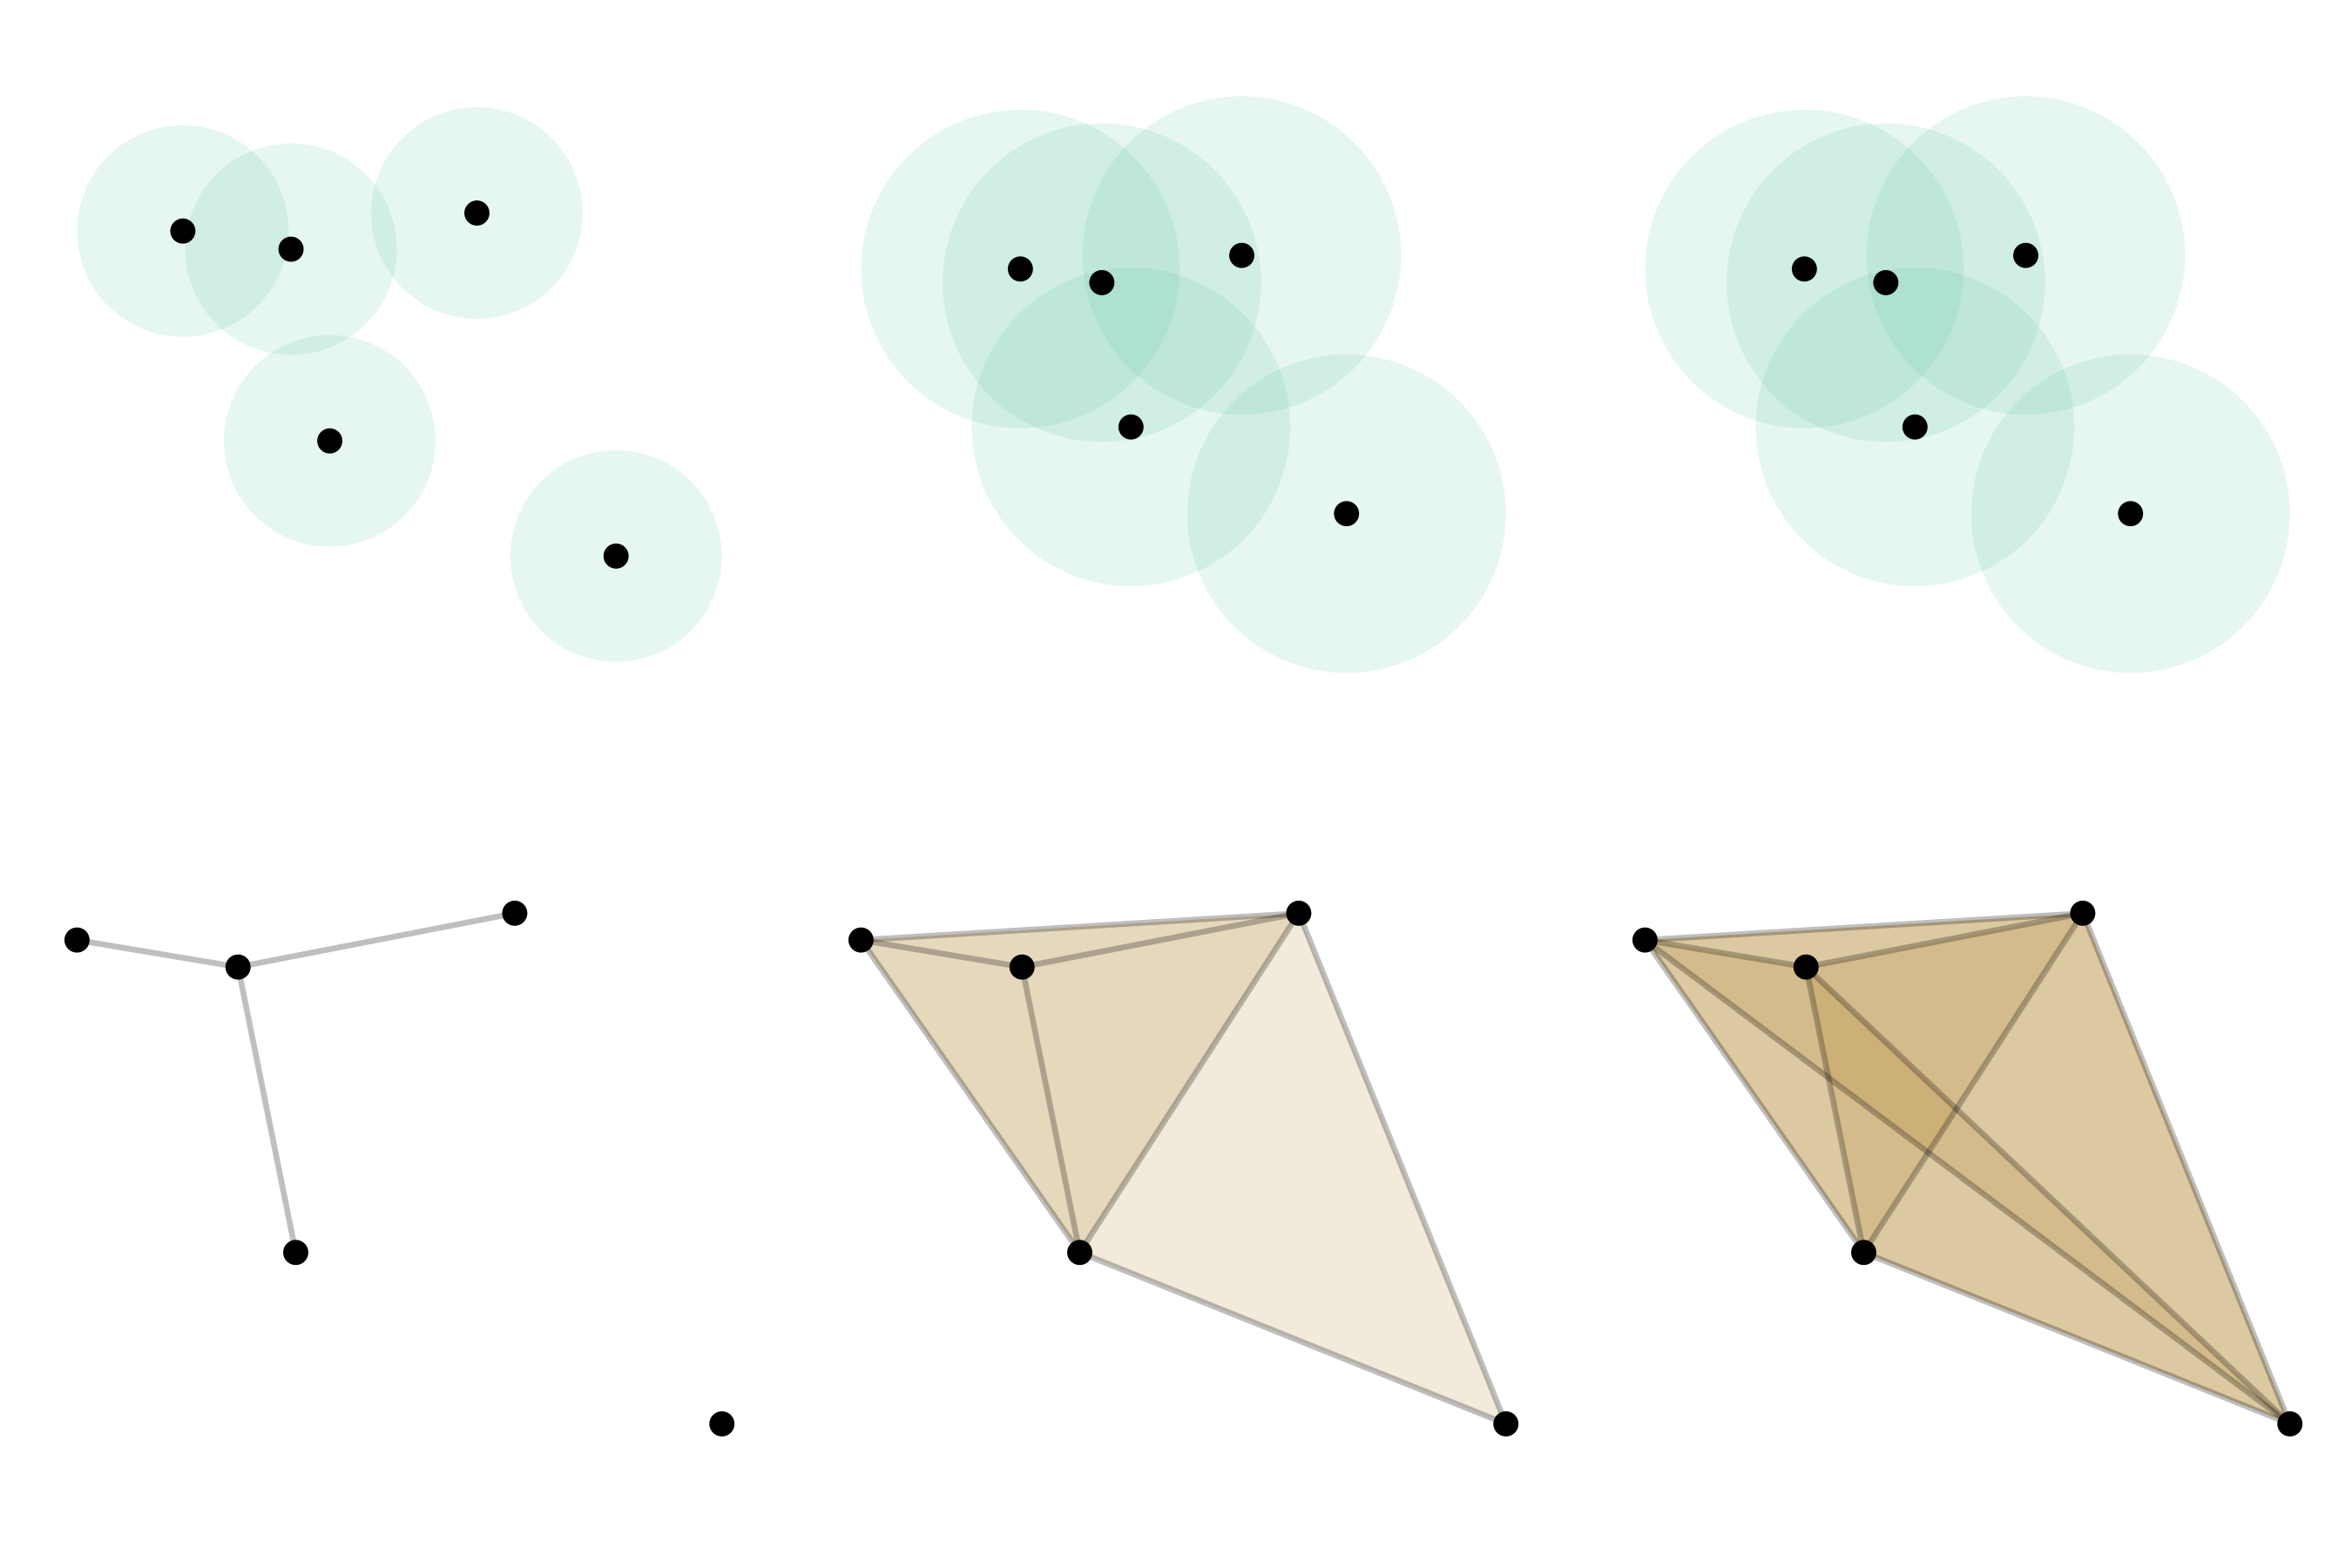
\includegraphics[width=1\linewidth,height=0.3\textheight]{fig1} \caption{The design of akc framework. Generally, the framework includes four steps, namely: (1) Keyword extraction (optional); (2) Keyword preprocessing; (3)   Network construction and clustering; (4)    Results presentation.}\label{fig:fig1}
\end{figure}

\begin{enumerate}
\def\labelenumi{(\arabic{enumi})}
\tightlist
\item
  Keyword extraction (optional)
\end{enumerate}

In bibliometric meta-data entries, the textual information of title, abstract and keyword are usually provided for each paper. If the keywords are used directly, there is no need to do information retrieval. Then we could directly skip this procedure and start from keyword preprocessing. However, sometimes the keyword field is missing, then we would need to extract the keywords from raw text in the title, abstract or full text with an external dictionary. At other times, one might want to get more keywords and their co-occurrence relationships from each entry. In such cases, the keyword field could serve as an internal dictionary for information retrieval in the provided raw text.

Figure \ref{fig:fig2} has displayed an example of keyword extraction procedure. First, the raw text would be split into sub-sentences (clauses), which suppresses the generation of cross-clause n-grams. Then the sub-sentences would be tokenized into n-grams. The \texttt{n} could be specified by the users, inspecting the average number of words in keyword phrases might help decide the maximum number of \texttt{n}. Finally, a filter is made. Only tokens that have emerged in the user-defined dictionary are retained for further analysis. The whole keyword extraction procedure could be implemented automatically with \texttt{keyword\_extract} function in \CRANpkg{akc}.

\begin{figure}
\includegraphics[width=1\linewidth,height=0.3\textheight]{fig2} \caption{An example of keyword extraction procedure. The raw text would be first divided sentence by sentence, then tokenized to n-grams and yield the target keywords based on a dictionary. The letters are automatically turned to lower case.}\label{fig:fig2}
\end{figure}

\begin{enumerate}
\def\labelenumi{(\arabic{enumi})}
\setcounter{enumi}{1}
\tightlist
\item
  Keyword preprocessing
\end{enumerate}

In practice, the textualized contents are seldom clean enough to implement analysis directly. Therefore, the upstream data cleaning process is inevitable. In keyword preprocessing procedure of \CRANpkg{akc} framework, the cleaning part would take care of some details in the preprocess, such as converting the letters to lower case and removing parentheses and contents inside (optional). For merging part, \CRANpkg{akc} help merge the synonymous phrases according to their lemmas or stems. While using lemmatization and stemming might get abnormal knowledge tokens, here in \CRANpkg{akc} we have designed a conversion rule to tackle this problem. We first get the lemmatized or stemmed form of keywords, then group them by their lemma or stem, and use the most frequent keyword in the group to represent the original keyword. This step could be realized by \texttt{keyword\_merge} function in \CRANpkg{akc} package. An example could be found in Table \ref{tab:tab1-2}. After keyword merging, there might still be too many keywords included in the analysis, which poses a great burden for computation in the subsequent procedures. Therefore, a filter should be carried out here, it could exclude the infrequent terms, or extract top TF-IDF terms, or use any criteria that meets the need. Last, a manual validation should be carried out to ensure the final data quality.

\begin{table}

\caption{\label{tab:tab1-2}An example of keyword merging rule applied in akc. The keywords with the same lemma or stem would be merged to the highest frequency keyword in the original form.}
\centering
\fontsize{7}{9}\selectfont
\begin{tabular}[t]{c|c|c|c}
\hline
ID & Original form & Lemmatized form & Merged form\\
\hline
1 & higher education & high education & higher education\\
\hline
2 & higher education & high education & higher education\\
\hline
3 & high educations & high education & higher education\\
\hline
4 & higher educations & high education & higher education\\
\hline
5 & high education & high education & higher education\\
\hline
6 & higher education & high education & higher education\\
\hline
\end{tabular}
\end{table}

\begin{enumerate}
\def\labelenumi{(\arabic{enumi})}
\setcounter{enumi}{2}
\tightlist
\item
  Network construction and clustering
\end{enumerate}

Based on keyword co-occurrence relationship, the keyword pairs would form an edge list for construction of an undirected network. Then the facilities provided by the \CRANpkg{igraph} package would automatically group the nodes (representing the keywords). This procedure could be achieved by using \texttt{keyword\_group} function in \CRANpkg{akc}.

\begin{enumerate}
\def\labelenumi{(\arabic{enumi})}
\setcounter{enumi}{3}
\tightlist
\item
  Results presentation
\end{enumerate}

Currently, there are two kinds of output presented by \CRANpkg{akc}. One is a summarized result, namely a table with group number and keyword collections (attached with frequency). Another is network visualization, which has two modes. The local mode provides a keyword co-occurrence network by group (use facets in \CRANpkg{ggplot2}), whereas the global mode displays the whole network structure. Note that one might include a huge number of keywords and make a vast network, but for presentation the users could choose how many keywords from each group to be displayed. More details could be found in the following sections.

The \CRANpkg{akc} framework could never be built without the powerful support provided by R community. The \CRANpkg{akc} package was developed under R environment, and main packages imported to \CRANpkg{akc} framework include \CRANpkg{data.table} (Dowle and Srinivasan 2021) for high-performance computing, \CRANpkg{dplyr} (Wickham et al. 2022) for tidy data manipulation, \CRANpkg{ggplot2} (Wickham 2016) for data visualization, \CRANpkg{ggraph} (Pedersen 2021) for network visualization, \CRANpkg{ggwordcloud} (Le Pennec and Slowikowski 2019) for word cloud visualization, \CRANpkg{igraph} (Csardi, Nepusz, et al. 2006) for network analysis, \CRANpkg{stringr} (Wickham 2019) for string operations, \CRANpkg{textstem} (Rinker 2018) for lemmatizing and stemming, \CRANpkg{tidygraph} (Pedersen 2022) for network data manipulation and \CRANpkg{tidytext} (Silge and Robinson 2016) for tidy tokenization. Getting more understandings on these R packages could help users utilize more alternative functions, so as to complete more specific and complex tasks. Hopefully, the users might also become potential developers of the \CRANpkg{akc} framework in the future.

\hypertarget{example}{%
\section{Example}\label{example}}

This section shows how \CRANpkg{akc} can be used in a real case. A collection of bibliometric data of \emph{R Journal} from 2009 to 2021 is used in this example. The data of this example can be accessed in the \href{https://github.com/hope-data-science/RJ_akc}{GitHub repository}. Only the \CRANpkg{akc} package is used in this workflow. First, we would load the package and import the data in the R environment.

\begin{verbatim}
library (akc)
rj_bib = readRDS ("./rj_bib.rds")
rj_bib
\end{verbatim}

\begin{verbatim}
#> # A tibble: 568 x 4
#>       id title                                                     abstr~1  year
#>    <int> <chr>                                                     <chr>   <dbl>
#>  1     1 Aspects of the Social Organization and Trajectory of the~ Based ~  2009
#>  2     2 asympTest: A Simple R Package for Classical Parametric S~ asympT~  2009
#>  3     3 ConvergenceConcepts: An R Package to Investigate Various~ Conver~  2009
#>  4     4 copas: An R package for Fitting the Copas Selection Model This a~  2009
#>  5     5 Party on!                                                 Random~  2009
#>  6     6 Rattle: A Data Mining GUI for R                           Data m~  2009
#>  7     7 sos: Searching Help Pages of R Packages                   The so~  2009
#>  8     8 The New R Help System                                     Versio~  2009
#>  9     9 Transitioning to R: Replicating SAS, Stata, and SUDAAN A~ Statis~  2009
#> 10    10 Bayesian Estimation of the GARCH(1,1) Model with Student~ This n~  2010
#> # ... with 558 more rows, and abbreviated variable name 1: abstract
\end{verbatim}

\texttt{rj\_bib} is a data frame with four columns, including \emph{id} (Paper ID), \emph{title} (Title of paper), \emph{abstract} (Abstract of paper) and \emph{year} (Publication year of paper). Papers in \emph{R Journal} do not contain a keyword field, thus we have to extract the keywords from the title or abstract field (first step in Figure \ref{fig:fig1}). Here in our case, we use the abstract field as our data source. In addition, we need a user-defined dictionary to extract the keywords, otherwise all the n-grams (meaningful or meaningless) would be extracted and the results would include redundant noise.

\begin{verbatim}
# import the user-defined dictionary
rj_user_dict = readRDS ("./rj_user_dict.rds")
rj_user_dict
\end{verbatim}

\begin{verbatim}
#> # A tibble: 627 x 1
#>    keyword            
#>    <chr>              
#>  1 seasonal-adjustment
#>  2 unit roots         
#>  3 transformations    
#>  4 decomposition      
#>  5 combination        
#>  6 integration        
#>  7 competition        
#>  8 regression         
#>  9 accuracy           
#> 10 symmetry           
#> # ... with 617 more rows
\end{verbatim}

Note that the dictionary should be a data.frame with only one column named ``keyword''. The user can also use \texttt{make\_dict} function to build the dictionary data.frame with a string vector. This function removes duplicated phrases, turns them to lower case and sorts them, which potentially improves the efficiency for the following processes.

\begin{verbatim}
rj_dict = make_dict (rj_user_dict$keyword)
\end{verbatim}

With the bibliometric data (\texttt{rj\_bib}) and dictionary data (\texttt{rj\_dict}), we could start the workflow provided in Figure \ref{fig:fig1}.

\begin{enumerate}
\def\labelenumi{(\arabic{enumi})}
\tightlist
\item
  Keyword extraction
\end{enumerate}

In this step, we need a bibliometric data table with simply two informative columns, namely paper ID (\emph{id}) and the raw text field (in our case \emph{abstract}). The parameter \emph{dict} is also specified to extract only keywords emerging in the user-defined dictionary. The implementation is very simple.

\begin{verbatim}
rj_extract_keywords = rj_bib %>% 
  keyword_extract (id = "id",text = "abstract",dict = rj_dict)
\end{verbatim}

By default, only phrases ranging 1 to 4 in length are included as extracted keywords. The user can change this range using parameters \texttt{n\_min} and \texttt{n\_max} in \texttt{keyword\_extract} function. These is also a \texttt{stopword} parameter, allowing users to exclude specific keywords in the extracted phrases. The output of \texttt{keyword\_extract} is a data.frame (tibble,\texttt{tbl\_df} class provided by \CRANpkg{tibble} package) with two columns, namely paper ID (\emph{id}) and the extracted keyword (\emph{keyword}).

\begin{enumerate}
\def\labelenumi{(\arabic{enumi})}
\setcounter{enumi}{1}
\tightlist
\item
  Keyword preprocessing
\end{enumerate}

For the preprocessing part, \texttt{keyword\_clean} and \texttt{keyword\_merge} would be implemented in the cleaning part and merging part respectively. In the cleaning part, the \texttt{keyword\_clean} function would: 1) Splits the text with separators (If no separators exist, skip); 2) Removes the contents in the parentheses (including the parentheses, optional); 3) Removes white spaces from start and end of string and reduces repeated white spaces inside a string; 4) Removes all the null character string and pure number sequences (optional); 5) Converts all letters to lower case; 6) Lemmatization (optional). The merging part has been illustrated in the previous section (see Table \ref{tab:tab1-2}), thus would not be explained again. In the tidy workflow, the preprocessing is implemented via:

\begin{verbatim}
rj_cleaned_keywords = rj_extract_keywords %>% 
  keyword_clean () %>% 
  keyword_merge ()
\end{verbatim}

No parameters are used in these functions because \CRANpkg{akc} has been designed to input and output tibbles with consistent column names. If the users have data tables with different column names, specify them in arguments (\texttt{id} and \texttt{keyword}) provided by the functions. More details can be found in the help document (use \texttt{?keyword\_clean} and \texttt{?keyword\_merge} in the console).

\begin{enumerate}
\def\labelenumi{(\arabic{enumi})}
\setcounter{enumi}{2}
\tightlist
\item
  Network construction and clustering
\end{enumerate}

To construct a keyword co-occurrence network, only a data table with two columns (with paper ID and keyword) is needed. All the details have been taken care of in the \texttt{keyword\_group} function. However, the user could specify: 1) the community detection function (use \texttt{com\_detect\_fun} argument); 2) the filter rule of keywords according to frequency (use \texttt{top} or \texttt{min\_freq} argument, or both). In our example, we would use the default settings (utilizing Fastgreedy algorithm, only top 200 keywords by frequency would be included).

\begin{verbatim}
rj_network = rj_cleaned_keywords %>% 
  keyword_group ()
\end{verbatim}

The output object \texttt{rj\_network} is a \texttt{tbl\_graph} class supported by \CRANpkg{tidygraph}, which is a tidy data format containing the network data. Based on this data, we can present the results in various forms in the next section.

\begin{enumerate}
\def\labelenumi{(\arabic{enumi})}
\setcounter{enumi}{3}
\tightlist
\item
  Results presentation
\end{enumerate}

Currently, there are two major ways to display the classified results in \CRANpkg{akc}, namely network and table. A fast way to gain the network visualization is using \texttt{keyword\_vis} function:

\begin{verbatim}
rj_network %>% 
  keyword_vis ()
\end{verbatim}

\begin{figure}

{\centering 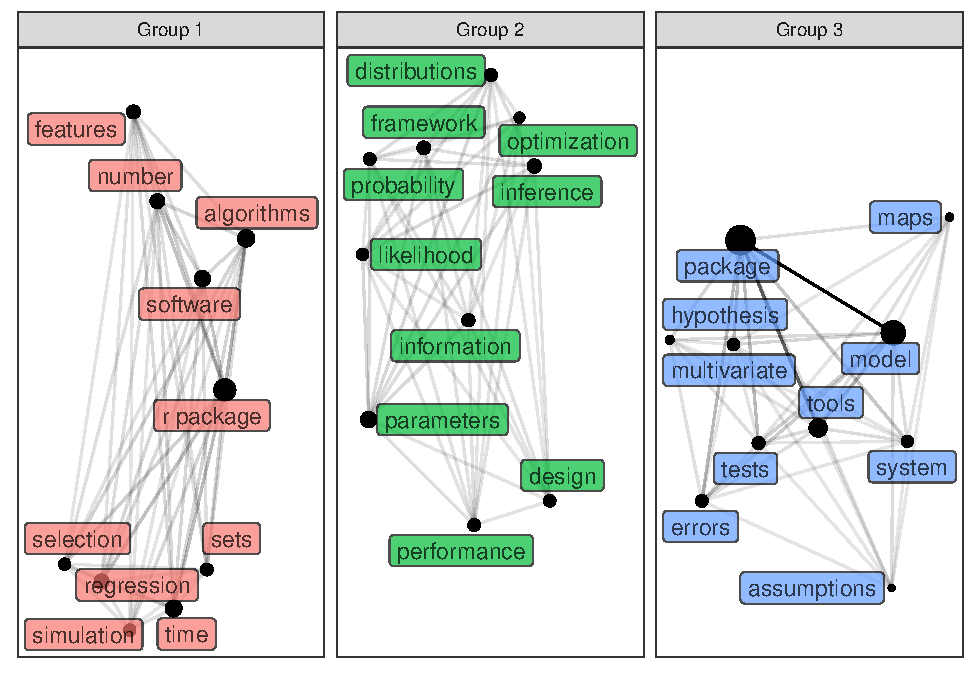
\includegraphics[width=1\linewidth]{RJ-2022-025_files/figure-latex/fig4-1} 

}

\caption{Network visualization for knowledge classification of R Journal (2009-2021). The keywords were automatically classified into three groups based on Fastgreedy algorithm. Only the top 10 keywords by frequency are displayed in each group.}\label{fig:fig4}
\end{figure}

In Figure \ref{fig:fig4}, the keyword co-occurrence network is clustered into three groups. The size of nodes is proportional to the keyword frequency, while the transparency degree of edges is proportional to the co-occurrence relationship between keywords. For each group, only the top 10 keywords by frequency are showed in each facet. If the user wants to dig into Group 1, \texttt{keyword\_network} could be applied. Also, \texttt{max\_nodes} parameter could be used to control how many nodes to be showed (in our case, we show 20 nodes in the visualization displayed in Figure \ref{fig:fig5}).

\begin{verbatim}
rj_network %>% 
  keyword_network (group_no = 1,max_nodes = 20) 
\end{verbatim}

\begin{figure}

{\centering 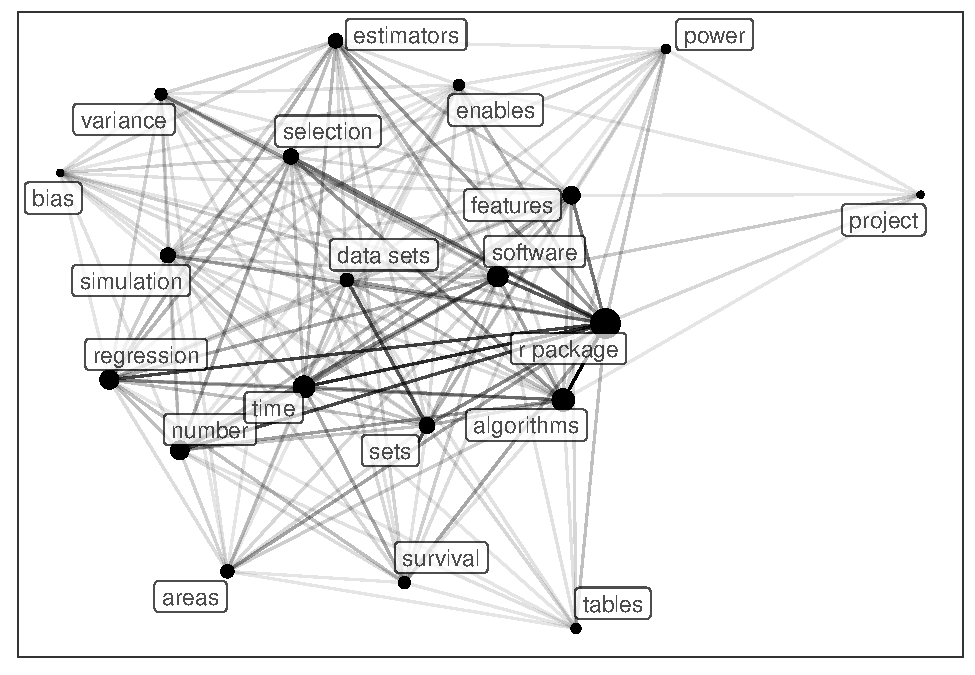
\includegraphics[width=1\linewidth]{RJ-2022-025_files/figure-latex/fig5-1} 

}

\caption{Focus on one cluster of the knowledge network of R journal (2009-2021). Top 20 keywords by frequency are shown in the displayed group.}\label{fig:fig5}
\end{figure}

Another displayed form is using table. This could be implemented by \texttt{keyword\_table} via:

\begin{verbatim}
rj_table = rj_network %>% 
  keyword_table () 
\end{verbatim}

This would return a data.frame with two columns (see Table \ref{tab:tab2-2}), namely the group number and the keywords (by default, only the top 10 keywords by frequency would be displayed, and the frequency information is attached).

\begin{table}

\caption{\label{tab:tab2-2}Top 10 keywords by frequency in each knowledge classification of R Journal (2009-2021).}
\centering
\fontsize{7}{9}\selectfont
\begin{tabular}[t]{c|>{\centering\arraybackslash}p{10cm}}
\hline
Group & Keywords (TOP 10)\\
\hline
1 & r package (238); algorithms (117); time (109); software (93); regression (75); number (72); features (60); sets (45); selection (41); simulation (40)\\
\hline
2 & parameters (98); inference (65); framework (58); information (51); distributions (48); performance (47); probability (45); design (44); likelihood (41); optimization (31)\\
\hline
3 & package (505); model (310); tools (140); tests (48); errors (46); multivariate (42); system (41); hypothesis (18); maps (16); assumptions (15)\\
\hline
\end{tabular}
\end{table}

Word cloud visualization is also supported by \CRANpkg{akc} via \CRANpkg{ggwordcloud} package, which could be implemented by using \texttt{keyword\_cloud} function.

In our example, we assume \emph{R Journal} has a large focus on introducing R packages (Group 1 and Group 3 contains ``r package'' and ``package'' respectively). Common statistical subjects mentioned in \emph{R Journal} include ``regression'' (in Group 1), ``optimization'' (in Group 2) and ``multivariate'' (in Group 3). While our example provides a preliminary analysis of knowledge classification in \emph{R Journal}, an in-depth exploration could be carried out with a more professional dictionary containing more relevant keywords, and more preprocessing could be implemented according to application scenarios (e.g.~``r package'' and ``package'' could be merged into one keyword, and unigrams could be excluded if we consider them carrying indistinct information).

\hypertarget{discussion}{%
\section{Discussion}\label{discussion}}

The core functionality of the akc framework is to automatically group the knowledge pieces (keywords) using modularity-based clustering. Because this process is unsupervised, it can be difficult to evaluate the outcome of classification. Nevertheless, the default setting of community detection algorithm was selected after empirical tests via \href{https://cran.r-project.org/web/packages/akc/vignettes/Benchmarking.html}{benchmarking}. It was found that: 1) Edge betweenness and Spinglass algorithm are most time-consuming; 2) Edge betweenness and Walktrap algorithm could potentially find more local clusters in the network; 3) Label propagation could hardly divide the keywords into groups; 4) Infomap has high standard deviation of node number across groups. In the end, Fastgreedy was chosen as the default community detection algorithm in \CRANpkg{akc}, because its performance is relatively stable, and the number of groups increases proportionally with the network size.

Though \CRANpkg{akc} currently focuses on automatic knowledge classification based on community detection in keyword co-occurrence network, this framework is rather general in many natural language processing problems. One could utilize part of the framework to complete some specific tasks, such as word consolidating (using keyword merging) and n-gram tokenizing (using keyword extraction with a null dictionary), then export the tidy table and work in another environment. As long as the data follows the rule of tidy data format (Wickham et al. 2014; Silge and Robinson 2017), the \CRANpkg{akc} framework could be easily decomposed and applied in various circumstances. For instance, by considering the nationalities of authors as keywords, \CRANpkg{akc} framework could also investigate the international collaboration behavior in specific domain.

In the meantime, the \CRANpkg{akc} framework is still in active development, trying new algorithms to carry out better unsupervised knowledge classification under the R environment. The expected new directions include more community detection functions, new clustering methods, better visualization settings, etc. Note that except for the topology-based community detection approach considering graph structure of the network, there is still another topic-based approach considering the textual information of the network nodes (Ding 2011), such as hierarchical clustering (Newman 2003), latent semantic analysis (Landauer, Foltz, and Laham 1998) and Latent Dirichlet Allocation (Blei, Ng, and Jordan 2003). These methods are also accessible in R, the relevant packages could be found in the \href{https://cran.r-project.org/web/views/NaturalLanguageProcessing.html}{CRAN Task View: Natural Language Processing}. With the tidy framework, \CRANpkg{akc} could assimilate more nutrition from the modern R ecosystem, and move forward to create better reproducible open science schemes in the future.

\hypertarget{conclusion}{%
\section{Conclusion}\label{conclusion}}

In this paper, we have proposed a tidy framework of automatic knowledge classification supported by a collection of R packages integrated by \CRANpkg{akc}. While focusing on data mining based on keyword co-occurrence network, the framework also supports other procedures in data science workflow, such as text cleaning, keyword extraction and consolidating synonyms. Though in the current stage it aims to support analysis in bibliometric research, the framework is quite flexible to extend to various tasks in other fields. Hopefully, this work could attract more participants from both R community and academia to get involved, so as to contribute to the flourishing open science in text mining.

\hypertarget{acknowledgement}{%
\section{Acknowledgement}\label{acknowledgement}}

This study is funded by The National Social Science Fund of China ``Research on Semantic Evaluation System of Scientific Literature Driven by Big Data'' (21\&ZD329). The source code and data for reproducing this paper can be found at: \url{https://github.com/hope-data-science/RJ_akc}.

\hypertarget{references}{%
\section*{References}\label{references}}
\addcontentsline{toc}{section}{References}

\hypertarget{refs}{}
\begin{CSLReferences}{1}{0}
\leavevmode\vadjust pre{\hypertarget{ref-8620850}{}}%
Amrahov, S. E., and B. Tugrul. 2018. {``A Community Detection Algorithm on Graph Data.''} In \emph{2018 International Conference on Artificial Intelligence and Data Processing (IDAP)}, 1--4.

\leavevmode\vadjust pre{\hypertarget{ref-BaziyadShirazi-628}{}}%
Baziyad, Hamed, Saeed Shirazi, Seyedmohammadreza Hosseini, and Rasoul Norouzi. 2019. {``Mapping the Intellectual Structure of Epidemiology with Use of Co-Word Analysis.''} \emph{Journal of Biostatistics and Epidemiology}.

\leavevmode\vadjust pre{\hypertarget{ref-Benoit2018}{}}%
Benoit, Kenneth, Kohei Watanabe, Haiyan Wang, Paul Nulty, Adam Obeng, Stefan Müller, and Akitaka Matsuo. 2018. {``{quanteda: An R package for the quantitative analysis of textual data}.''} \emph{Journal of Open Source Software} 3 (30): 774.

\leavevmode\vadjust pre{\hypertarget{ref-BleiNg-634}{}}%
Blei, David M., Andrew Y. Ng, and Michael I. Jordan. 2003. {``Latent Dirichlet Allocation.''} \emph{Journal of Machine Learning Research} 3: 993--1022.

\leavevmode\vadjust pre{\hypertarget{ref-Blondel_2008}{}}%
Blondel, Vincent D, Jean-Loup Guillaume, Renaud Lambiotte, and Etienne Lefebvre. 2008. {``Fast Unfolding of Communities in Large Networks.''} \emph{Journal of Statistical Mechanics: Theory and Experiment} 2008 (10): P10008.

\leavevmode\vadjust pre{\hypertarget{ref-callon1986mapping}{}}%
Callon, Michel, Arie Rip, and John Law. 1986. \emph{Mapping the Dynamics of Science and Technology: Sociology of Science in the Real World}. Springer.

\leavevmode\vadjust pre{\hypertarget{ref-chen2006citespace}{}}%
Chen, Chaomei. 2006. {``{CiteSpace II: Detecting and visualizing emerging trends and transient patterns in scientific literature}.''} \emph{Journal of the American Society for Information Science and Technology} 57 (3): 359--77.

\leavevmode\vadjust pre{\hypertarget{ref-Clauset}{}}%
Clauset, Aaron, M. E. J. Newman, and Cristopher Moore. 2004. {``Finding Community Structure in Very Large Networks.''} \emph{Physical Review E} 70 (December): 066111.

\leavevmode\vadjust pre{\hypertarget{ref-csardi2006igraph}{}}%
Csardi, Gabor, Tamas Nepusz, et al. 2006. {``The Igraph Software Package for Complex Network Research.''} \emph{InterJournal, Complex Systems} 1695 (5): 1--9.

\leavevmode\vadjust pre{\hypertarget{ref-Ding-629}{}}%
Ding, Ying. 2011. {``Community Detection: Topological Vs. Topical.''} \emph{Journal of Informetrics} 5 (4): 498--514.

\leavevmode\vadjust pre{\hypertarget{ref-dowle2021data}{}}%
Dowle, Matt, and Arun Srinivasan. 2021. \emph{Data.table: Extension of `Data.frame`}. \url{https://CRAN.R-project.org/package=data.table}.

\leavevmode\vadjust pre{\hypertarget{ref-Fortunato-627}{}}%
Fortunato, Santo. 2010. {``Community Detection in Graphs.''} \emph{Physics Reports} 486 (3): 75--174.

\leavevmode\vadjust pre{\hypertarget{ref-garg2017comparative}{}}%
Garg, Neha, and Rinkle Rani. 2017. {``{A comparative study of community detection algorithms using graphs and R}.''} In \emph{2017 International Conference on Computing, Communication and Automation (ICCCA)}, 273--78. IEEE.

\leavevmode\vadjust pre{\hypertarget{ref-girvan2002community}{}}%
Girvan, Michelle, and Mark EJ Newman. 2002. {``Community Structure in Social and Biological Networks.''} \emph{Proceedings of the National Academy of Sciences} 99 (12): 7821--26.

\leavevmode\vadjust pre{\hypertarget{ref-he1999knowledge}{}}%
He, Q. 1999. {``Knowledge Discovery Through Co-Word Analysis.''} \emph{Library Trends} 48 (1): 133--59.

\leavevmode\vadjust pre{\hypertarget{ref-hu2013co}{}}%
Hu, Chang-Ping, Ji-Ming Hu, Sheng-Li Deng, and Yong Liu. 2013. {``{A co-word analysis of library and information science in China}.''} \emph{Scientometrics} 97 (2): 369--82.

\leavevmode\vadjust pre{\hypertarget{ref-hu2015research}{}}%
Hu, Jiming, and Yin Zhang. 2015. {``{Research patterns and trends of Recommendation System in China using co-word analysis}.''} \emph{Information Processing \& Management} 51 (4): 329--39.

\leavevmode\vadjust pre{\hypertarget{ref-huang2019measuring}{}}%
Huang, Tian-Yuan, and Bin Zhao. 2019. {``Measuring Popularity of Ecological Topics in a Temporal Dynamical Knowledge Network.''} \emph{PloS One} 14 (1): e0208370.

\leavevmode\vadjust pre{\hypertarget{ref-JavedYounis-626}{}}%
Javed, Muhammad Aqib, Muhammad Shahzad Younis, Siddique Latif, Junaid Qadir, and Adeel Baig. 2018. {``{Community detection in networks: A multidisciplinary review}.''} \emph{Journal of Network and Computer Applications} 108: 87--111.

\leavevmode\vadjust pre{\hypertarget{ref-khasseh2017intellectual}{}}%
Khasseh, Ali Akbar, Faramarz Soheili, Hadi Sharif Moghaddam, and Afshin Mousavi Chelak. 2017. {``{Intellectual structure of knowledge in iMetrics: A co-word analysis}.''} \emph{Information Processing \& Management} 53 (3): 705--20.

\leavevmode\vadjust pre{\hypertarget{ref-kwasnik1999role}{}}%
Kwasnik, Barbara H. 1999. {``The Role of Classification in Knowledge Representation and Discovery.''} \emph{Library Trends} 48 (1): 22--47.

\leavevmode\vadjust pre{\hypertarget{ref-LandauerFoltz-635}{}}%
Landauer, Thomas K., Peter W. Foltz, and Darrell Laham. 1998. {``An Introduction to Latent Semantic Analysis.''} \emph{Discourse Processes} 25 (2-3): 259--84.

\leavevmode\vadjust pre{\hypertarget{ref-pennec2019ggwordcloud}{}}%
Le Pennec, Erwan, and Kamil Slowikowski. 2019. \emph{Ggwordcloud: A Word Cloud Geom for 'Ggplot2'}. \url{https://CRAN.R-project.org/package=ggwordcloud}.

\leavevmode\vadjust pre{\hypertarget{ref-leung2017bibliometrics}{}}%
Leung, Xi Y, Jie Sun, and Billy Bai. 2017. {``{Bibliometrics of social media research: A co-citation and co-word analysis}.''} \emph{International Journal of Hospitality Management} 66: 35--45.

\leavevmode\vadjust pre{\hypertarget{ref-li2017knowledge}{}}%
Li, Xinjian, Emily Ma, and Hailin Qu. 2017. {``{Knowledge mapping of hospitality research- A visual analysis using CiteSpace}.''} \emph{International Journal of Hospitality Management} 60: 77--93.

\leavevmode\vadjust pre{\hypertarget{ref-Mullen2018}{}}%
Mullen, Lincoln A., Kenneth Benoit, Os Keyes, Dmitry Selivanov, and Jeffrey Arnold. 2018. {``Fast, Consistent Tokenization of Natural Language Text.''} \emph{Journal of Open Source Software} 3 (23): 655.

\leavevmode\vadjust pre{\hypertarget{ref-Murata2010}{}}%
Murata, Tsuyoshi. 2010. {``Detecting Communities in Social Networks.''} In \emph{Handbook of Social Network Technologies and Applications}, edited by Borko Furht, 269--80. Boston, MA: Springer US.

\leavevmode\vadjust pre{\hypertarget{ref-Newman-633}{}}%
Newman, Mark EJ. 2003. {``The Structure and Function of Complex Networks.''} \emph{SIAM Review} 45 (2): 167--256.

\leavevmode\vadjust pre{\hypertarget{ref-newman2004fast}{}}%
---------. 2004. {``Fast Algorithm for Detecting Community Structure in Networks.''} \emph{Physical Review E} 69 (6): 066133.

\leavevmode\vadjust pre{\hypertarget{ref-newman2006finding}{}}%
---------. 2006. {``Finding Community Structure in Networks Using the Eigenvectors of Matrices.''} \emph{Physical Review E} 74 (3): 036104.

\leavevmode\vadjust pre{\hypertarget{ref-pedersen2021ggraph}{}}%
Pedersen, Thomas Lin. 2021. \emph{Ggraph: An Implementation of Grammar of Graphics for Graphs and Networks}. \url{https://CRAN.R-project.org/package=ggraph}.

\leavevmode\vadjust pre{\hypertarget{ref-pedersen2022tidygraph}{}}%
---------. 2022. \emph{Tidygraph: A Tidy API for Graph Manipulation}. \url{https://CRAN.R-project.org/package=tidygraph}.

\leavevmode\vadjust pre{\hypertarget{ref-pons2005computing}{}}%
Pons, Pascal, and Matthieu Latapy. 2005. {``Computing Communities in Large Networks Using Random Walks.''} In \emph{International Symposium on Computer and Information Sciences}, 284--93. Springer.

\leavevmode\vadjust pre{\hypertarget{ref-raghavan2007near}{}}%
Raghavan, Usha Nandini, Reka Albert, and Soundar Kumara. 2007. {``Near Linear Time Algorithm to Detect Community Structures in Large-Scale Networks.''} \emph{Physical Review E} 76 (3): 036106.

\leavevmode\vadjust pre{\hypertarget{ref-reichardt2006statistical}{}}%
Reichardt, Jorg, and Stefan Bornholdt. 2006. {``Statistical Mechanics of Community Detection.''} \emph{Physical Review E} 74 (1): 016110.

\leavevmode\vadjust pre{\hypertarget{ref-rinker2018textstem}{}}%
Rinker, Tyler W. 2018. \emph{{textstem}: Tools for Stemming and Lemmatizing Text}. Buffalo, New York. \url{http://github.com/trinker/textstem}.

\leavevmode\vadjust pre{\hypertarget{ref-rosvall2009map}{}}%
Rosvall, Martin, Daniel Axelsson, and Carl T Bergstrom. 2009. {``The Map Equation.''} \emph{The European Physical Journal Special Topics} 178 (1): 13--23.

\leavevmode\vadjust pre{\hypertarget{ref-rosvall2007information}{}}%
Rosvall, Martin, and Carl T Bergstrom. 2007. {``An Information-Theoretic Framework for Resolving Community Structure in Complex Networks.''} \emph{Proceedings of the National Academy of Sciences} 104 (18): 7327--31.

\leavevmode\vadjust pre{\hypertarget{ref-silge2016tidytext}{}}%
Silge, Julia, and David Robinson. 2016. {``{tidytext: Text Mining and Analysis Using Tidy Data Principles in R}.''} \emph{Journal of Open Source Software} 1 (3). \url{https://doi.org/10.21105/joss.00037}.

\leavevmode\vadjust pre{\hypertarget{ref-Julia-3165010}{}}%
---------. 2017. \emph{Text Mining with r: A Tidy Approach}. O'Reilly Media, Inc.

\leavevmode\vadjust pre{\hypertarget{ref-de2014evaluating}{}}%
Sousa, Fabiano Berardo de, and Liang Zhao. 2014. {``Evaluating and Comparing the Igraph Community Detection Algorithms.''} In \emph{2014 Brazilian Conference on Intelligent Systems}, 408--13. IEEE.

\leavevmode\vadjust pre{\hypertarget{ref-van2010software}{}}%
Van Eck, Nees Jan, and Ludo Waltman. 2010. {``Software Survey: VOSviewer, a Computer Program for Bibliometric Mapping.''} \emph{Scientometrics} 84 (2): 523--38.

\leavevmode\vadjust pre{\hypertarget{ref-wang2018three}{}}%
Wang, Mengyang, and Lihe Chai. 2018. {``Three New Bibliometric Indicators/Approaches Derived from Keyword Analysis.''} \emph{Scientometrics} 116 (2): 721--50.

\leavevmode\vadjust pre{\hypertarget{ref-wickham2014tidy}{}}%
Wickham, Hadley et al. 2014. {``Tidy Data.''} \emph{Journal of Statistical Software} 59 (10): 1--23.

\leavevmode\vadjust pre{\hypertarget{ref-wickham2016ggplot2}{}}%
Wickham, Hadley. 2016. \emph{Ggplot2: Elegant Graphics for Data Analysis}. Springer-Verlag New York. \url{https://ggplot2.tidyverse.org}.

\leavevmode\vadjust pre{\hypertarget{ref-wickham2019stringr}{}}%
---------. 2019. \emph{Stringr: Simple, Consistent Wrappers for Common String Operations}. \url{https://CRAN.R-project.org/package=stringr}.

\leavevmode\vadjust pre{\hypertarget{ref-wickham2022dplyr}{}}%
Wickham, Hadley, Romain Francois, Lionel Henry, Kirill Muller, et al. 2022. \emph{Dplyr: A Grammar of Data Manipulation}. \url{https://CRAN.R-project.org/package=dplyr}.

\leavevmode\vadjust pre{\hypertarget{ref-wickham2016r}{}}%
Wickham, Hadley, and Garrett Grolemund. 2016. \emph{R for Data Science: Import, Tidy, Transform, Visualize, and Model Data}. O'Reilly Media, Inc.

\leavevmode\vadjust pre{\hypertarget{ref-yang2016comparative}{}}%
Yang, Zhao, Rene Algesheimer, and Claudio J Tessone. 2016. {``A Comparative Analysis of Community Detection Algorithms on Artificial Networks.''} \emph{Scientific Reports} 6 (1): 1--18.

\end{CSLReferences}

\bibliography{akc.bib}

\address{%
Tian-Yuan Huang\\
National Science Library, Chinese Academy of Sciences\\%
Beijing, China\\
%
%
\textit{ORCiD: \href{https://orcid.org/0000-0002-4151-3764}{0000-0002-4151-3764}}\\%
\href{mailto:huangtianyuan@mail.las.ac.cn}{\nolinkurl{huangtianyuan@mail.las.ac.cn}}%
}

\address{%
Li Li\\
National Science Library, Chinese Academy of Sciences; Department of Library, Information and Archives Management, School of Economics and Management, University of Chinese Academy of Science\\%
Beijing, China\\
%
%
%
\href{mailto:lili2020@mail.las.ac.cn}{\nolinkurl{lili2020@mail.las.ac.cn}}%
}

\address{%
Liying Yang\\
National Science Library, Chinese Academy of Sciences\\%
Beijing, China\\
%
%
%
\href{mailto:yangly@mail.las.ac.cn}{\nolinkurl{yangly@mail.las.ac.cn}}%
}

\end{article}


\end{document}
